\section{Results}
Using the aforementioned analysis procedure we found resulting communities and their related collocations and SIPs for a number of search terms.

\subsection{Glenn Beck}
Glenn Beck is a controversial conservative cable television show host on the Fox News network.  We performed a strong pair search for users who used both ``Glenn'' and ``Beck'' in at least one directed tweet.  We then grew communities from the set of 38 user pairs that resulted using the recursive community growth algorithm.  We hoped that because of Glenn Beck's controversial nature we would be able to find distinct communities with little or no cross interaction.

\begin{figure}
  \begin{center}
  
\includegraphics[width=6in]{figures/gb5.pdf}
  \end{center}
  \caption{The full graph for one of the 5 major communities found for the the Glenn Beck search.  The node labeling indicates the user's unique Twitter ID.}
  \label{figure:gb-full}
\end{figure}

\begin{figure}
  \begin{center}
  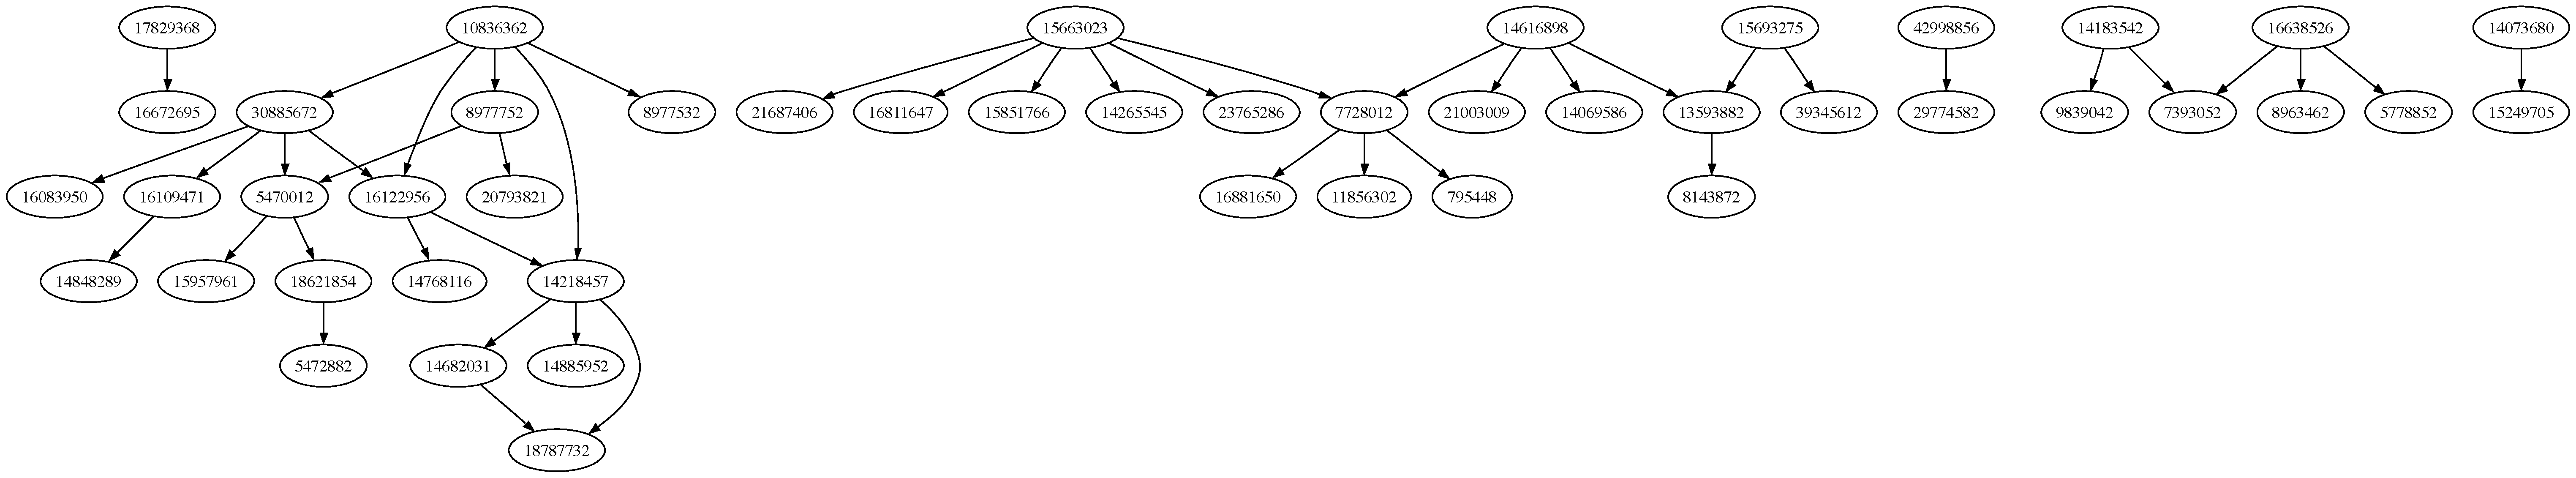
\includegraphics[width=6in]{figures/gb5-reduced.pdf}
  \end{center}
  \caption{The reduced graph for one of the 5 major communities found for the the Glenn Beck search.  Edges which did not meet a minimum weight were pruned from the graph.  If a node was unconnected after pruning it does not appear in the graph.  The node labeling indicates the user's unique Twitter ID.}
  \label{figure:gb-reduced}
\end{figure}

The full graph of the 5 interacting communities can be found in Figure figure:gbAppend, Appendix A, ``Full Glenn Beck Graph''.